\newtheorem{theo}{Theorem}
\newtheorem{lemma}{Lemma}
\newtheorem{col}{Corollary}
\newtheorem{defini}{Definition}
\newtheorem{pro}{Property}
\def\bm#1{\mbox{\boldmath{$#1$}}} \def\eqtri{\stackrel{\triangle}{=}}
\def\c#1{#1^{\dagger}} \newcommand{\gf}{\mbox{$GF(q)$}}
\newcommand{\av}[1]{\mbox{E${\displaystyle\left[ #1 \right]}$}} \def\r{\bm{r}}
\def\s{\bm{s}} \def\w{\bm{w}} \def\x{\bm{x}} \def\y{\bm{y}} \def\a{\bm{a}}
\def\u{\bm{u}} \def\cX{{\cal X}} \def\cY{{\cal Y}} \def\cP{{\cal P}}
\def\cV{{\cal V}} \newcommand{\g}{\mbox{$\Gamma$}}
\def\qed{\strut\hfill(Q.E.D.)} \def\eot{\strut\hfill$\Box$}
\def\osum{\bigcirc\hspace{-1.2em}\sum} \newcommand{\vt}[1]{\mbox{\boldmath
$#1$}}

\chapter{Introduction}
This chapter introduces the necessary background to conduct research on
dimensional speech emotion recognition. The aims, problems, concept,
contributions, and structure of the dissertation are also briefly presented as
guide in navigating the following chapters.

\section{Background}
Emotion can be regarded as the major difference between humans and computers.
At the beginning of human-computer interaction (HCI) development, no computer
would understand human emotion. Nowadays, there have been attempted to
recognize human emotion automatically by computers. If a computer could
correctly recognize emotion, HCI would be benefited greatly. For example, 
vehicle could detect driver's mood (long time emotion) to ensure safety. In
other applications, the satisfaction and performance of user and operator
through call center applications can be measured using speech emotion
recognition technologies.

Speech emotion recognition (SER) is an emerging technology that is resulted
from science in multi-discipline area, including psychology, physiology,
acoustics, and affective computing. The psychology of emotion focuses on how a
human reacts to certain stimuli and how these stimuli affect both mentally and
physically of humans. The physiology of emotion is related to arousal of the
nervous system with various states and strengths of arousal relating to
particular emotions. The acoustic of emotion studies on what acoustic features
relate to human emotion. The latter affective computing, according to Picard
\cite{Picard}, is termed as ``computing that relates to, arises from, or
influences emotion."

% add definition and rationale for linguistic information
Aside from those disciplines, language also has an impact on the expression of
emotion. Humans communicate emotion through speech and language
\cite{Kotz2011}. Furthermore,  language is argued to shape perceived emotion
intrinsically \cite{Lindquist2006}. Thus, utilizing linguistic information in
automatic SER may be useful to make computer accurately recognize human
emotions. 

% add definition of information science
Information science is a study of using information processing to find a
solution to an important social problem. In information science, a hierarchy of
data-information-knowledge (DIK) is known to model the flow of data. This model
can be used to model emotion recognition. The input to the data is signal,
which is an acoustic signal in SER. The data is the speech dataset. The
information is the features (acoustic and linguistic). The knowledge is the
degree of dimensional emotion. This concept, which will be explained in more
detail in Chapter 3, correlates information science with SER or models SER from
an information science perspective. 

% acoustic information science
Acoustic information science is the study of information science for acoustic
phenomena -- phenomena relate to sound. Speech is part of acoustic information
science; thus, the study of speech involves concepts used in acoustic
information science (e.g., acoustic signal processing). SER, although
multidisciplinary research, involves two main fields, the acoustics of speech
and the psychology of emotion. For automatic SER by computers, the
understanding of speech acoustics and computer algorithms will provide a
necessary foundation for building a better SER system.

% Back to SER, why studying SER with multidisciplinary research
This experimental study explores the necessity of fusing acoustic and
linguistic information for dimensional emotion recognition. The study views SER
from an acoustic information science point of view. Speech contains both
linguistic (verbal) and acoustic (non-verbal) information. While the
conventional SER method only uses acoustic information, fusing both acoustic
and linguistic information exists in human-human communication and is feasible
for human-computer interaction.

\section{Research aims and problems}
Speech is the primary modality for communication (known as speech
communication) including communicating human emotions. Even if other modalities
may influence on how human communicate emotions (e.g., facial expressions,
gesture, posture, body's motion/movement, and other physiological signals), in
special cases, like in telephone calls or voice assistant applications, 
speech is the only modality to determine a speaker's emotion.

In certain cases, using acoustic information only (e.g., prosody or intonation)
to perceive human emotions may be not enough. For instance, happy and angry
voices may have similarities in high intonation, sad and fear may have
similarities in low intonations. In this case, knowing the semantic of the
spoken words will increase the probability to recognize the perceived emotion
from speech. If the words have positive meanings and are uttered with high
intonations, then the chance that the speaker was happy is higher than angry.
This bimodal information fusion of acoustic and linguistic could be implemented
in computer algorithms to improve the performance of SER.

Thus, combining acoustic and linguistic information is relevant for improving
SER performance by computers. There is no need to add additional modalities
since linguistic information can be derived from speech. Modern automatic
speech recognition (ASR) can produce text in almost real-time processing. The
transcribed spoken text can be used to extract linguistic information. Both
acoustic and linguistic information can be fused in such frameworks to evaluate
the effectiveness of information fusion over unimodal information.

The main goal of this research is to investigate the necessity of fusing
acoustic information with linguistic information for dimensional SER. To
achieve this main goal, the following three sub-goals were addressed: 
\begin{enumerate}
\item maximizing the potency of SER from acoustic information only by
investigating the region of analysis and silence region for feature extraction,
\item studying the fusion of acoustic and linguistic information at the feature
level (early fusion) and its effect, particularly for valence prediction
improvement, and 
\item studying the fusion of acoustic and linguistic information at the decision
level (late fusion) and comparing the results with the previous approach.  
\end{enumerate}

There are five problems to be solved by these goals. The first problem is the
region of analysis for acoustic feature extraction. The second problem is the
effect of silent pause region in dimensional SER. The third problem is the low
performance of valence prediction. The fourth problem is the necessity to fuse
acoustic information and linguistic information for dimensional SER. The fifth
problem is to find the effective fusion framework for combining acoustic and
linguistic information. Figure \ref{fig:aims_issues} shows the connections
between research aims and research problems. The details of these aims (which
is transformed into research strategies) and problems (issues) are discussed
further in Chapter 3. 

\begin{figure}[htbp]
    \centering
    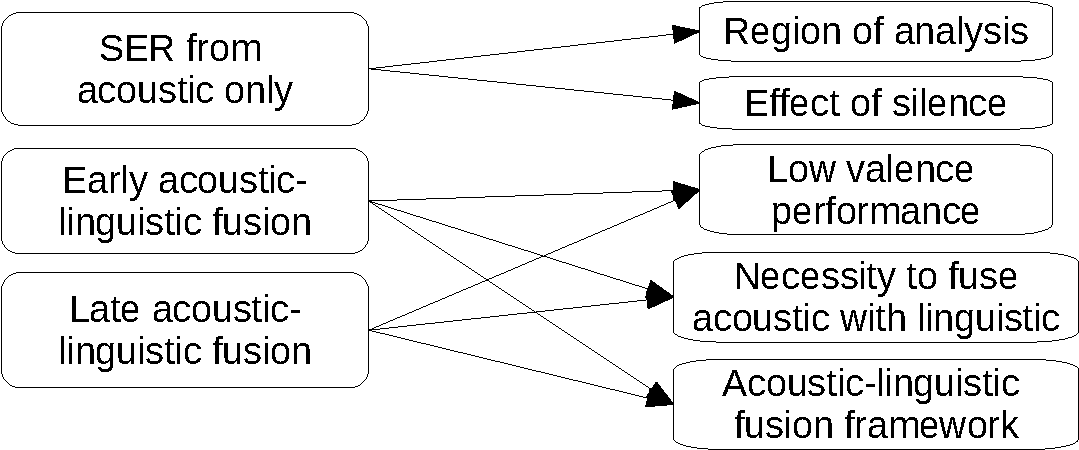
\includegraphics[width=0.7\textwidth]{../fig/aims_issues-crop.pdf}
    \caption{Connection between research aims (left) and research problems (right)}
    \label{fig:aims_issues}
\end{figure}

\section{Research concept}
% explains research concept: speech is not only about how but what
Speech delivers a message that goes beyond words. In this understanding, word
meaning is not enough to convey a message; acoustic information is needed.
Acoustic information alone is also not enough to deliver a message. It is not
only how it is said (acoustic), but also what is said (linguistic).
This concept is the foundation of this research, shown in Figure
\ref{fig:concept}. 

\begin{figure}[htbp]
    \centering
    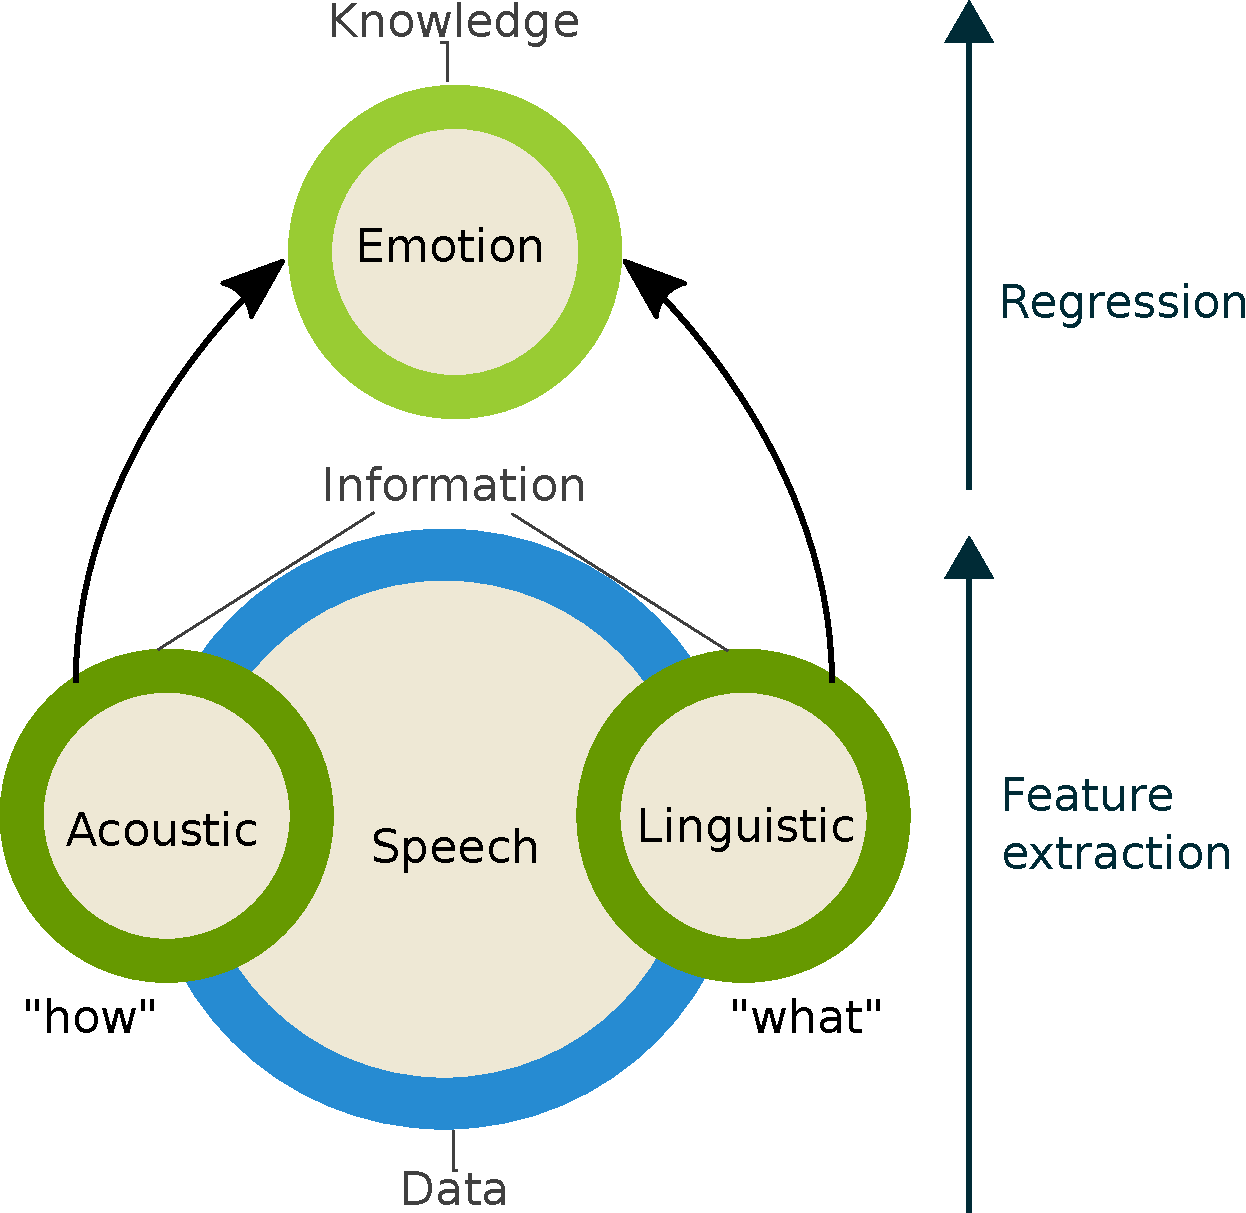
\includegraphics[width=0.6\textwidth]{../fig/concept-rev.pdf}
    \caption{Research concept of dimensional speech emotion recognition by fusing acoustic and linguistic information}
    \label{fig:concept}
\end{figure}

This research concept differs from the previous studies (e.g., \cite{Li2019b,
Vayrynen2014}). In these studies, the belief for speech is about how it is said
rather than what is said. This study combines both ``how'' and ``what''
information. Acoustic features contain information on how it is being said.
Linguistic features contain information on what is being said. Fusing both
pieces of information, which are extracted from a speech, will improve the
clarity of the message, including the expressed emotion. The perception of
emotion will also improve by fusing this bimodal information. Figure
\ref{fig:concept} shows the concept of automatic recognition of dimensional SER
by fusing both pieces of information. This process is also in line with the
previous DIK concept in information science.

The process of recognizing emotion from speech consists of two main steps.
First is extracting information from speech data; second is extracting degree
of dimensional emotions as knowledge from acoustic and linguistic information.
Features extraction extracts two pieces of information from speech --- acoustic
and linguistic. Since dimensional SER is a regression task, a regression
process will map extracted features to the ground truth labels. This process is
commonly performed within machine learning or deep learning. The acoustic and
linguistic information are fused in this step, which can be implemented in
various ways.

\section{Contributions}
The contributions of this dissertation can be traced to the published papers.
These contributions can be divided into three areas, as follows.
\begin{enumerate}
\item Acoustic feature extraction \\
In \cite{Atmaja2019} the author evaluated categorical speech emotion
recognition from silence-removed speech region. The result suggests that
extracting acoustic features from the silence-removed region is better than
from the whole speech region. In \cite{Atmaja2020f}, the author utilized
silence as an additional feature to statistical functions. The results achieved
a better score than baseline raw speech. The author confirms and generalizes
the effectiveness of mean and standard deviations of low-level acoustic
features for SER \cite{Atmaja2020f, Atmaja2020d}. In \cite{Atmaja2020h}, the
author showed that acoustic feature aggregation leads to better performances
than output aggregation. These contributions are explained in Chapter 4. In
\cite{Atmaja2020j}, the author found that the acoustic features that perform
better in SER will also perform better in song emotion recognition.

\item Information fusion \\
In \cite{Atmaja2019b, Atmaja2020d, Atmaja2020h}, the author proposed emotion
recognition by fusing acoustic and linguistic information at feature level. The
results significantly improved unimodal dimensional emotion recognition from
either acoustic or linguistic information. Furthermore, the author discussed the
improvement of valence prediction in \cite{Atmaja2020e}. While this
contribution is discussed in Chapter 5, the improved version of the proposed
method, the late fusion method, is explained in Chapter 6. The evaluated fusion
methods are expanded not only for acoustic and linguistic fusion but also for
acoustic and visual information fusion \cite{Atmaja2020, Elbarougy2020}. 

\item Classification methods \\ 
Modern classification methods utilized deep learning models. However, the
conventional method, such as support vector machine (SVM) and multi-layer
perceptron (MLP), are still used in many fields. The author showed that
traditional MLP with deeper layers and proper configurations performed better
than modern deep learning architecture \cite{Atmaja2020k}. For the SER task
with deep learning, the author confirmed the need for bigger data size to be fed
to deep learning models \cite{Atmaja2019c}. The choice of the loss function is
a matter in machine/deep learning. The author proposed correlation-based loss
function to improve the performance of dimensional SER \cite{Atmaja2020,
Atmaja2020d,Atmaja2020b}. The author also evaluated multitask learning (MTL)
for predicting valence, arousal, and dominance degrees simultaneously based on
this loss function \cite{Atmaja2020d, Atmaja2020i}.  Furthermore, the author
found that recurrent-based neural networks (RNN) are effective for the SER task
\cite{Atmaja2019a}. More improvements were obtained when this RNN model is
combined with the attention model \cite{Atmaja2019}.
\end{enumerate}


\section{Dissertation structure}
This dissertation is organized in eight chapters. The rest of these chapters is
organized as follows.
% a visualisation of this structure is
% illustrated in Figure \ref{fig:dissertation_org}.
\begin{itemize}
\item \textbf{Chapter 2} presents a literature study on speech emotion
recognition from bimodal acoustic and linguistic information fusion. An
introduction that motivates the previous research by fusing acoustic and
linguistic information is presented. This chapter reviews the models, features,
classifiers, and fusion methods for the SER task.
\item \textbf{Chapter 3} describes the research methodology --- justification
for using particular research methods. This chapter consists of the motivation
of researching SER, research issues, research philosophy, research strategies,
datasets, and a description of an evaluation metric. 
\item \textbf{Chapter 4} describes SER by using acoustic features. This chapter
investigates the region of analysis, the effect of silent pause features, and
the aggregation methods for acoustic-based SER.
\item \textbf{Chapter 5} describes the fusion of acoustic and linguistic
information at the feature level. This chapter evaluates the concatenation of
features and networks for bimodal emotion recognition from acoustic and
linguistic information. A SER evaluation from automatic transcription is also
provided in addition to manual transcription.
\item \textbf{Chapter 6} describes the fusion of acoustic and linguistic
information at the decision level. This chapter evaluates the late-fusion
approach by combining both information on two steps processing, including some
related issues: speaker-dependent vs. speaker-independent scenarios and effect
of lexical-controlled lexicons.
\item \textbf{Chapter 7} compares the results within this study and with other
studies. 
\item \textbf{Chapter 8} presents the overall conclusions of the dissertation.
Some possible future research directions are proposed from the current research
findings.
\end{itemize}

This dissertation's organization is summarized in Figure
\ref{fig:dissertation_org}. 

\begin{figure}[htbp]
    \centering
    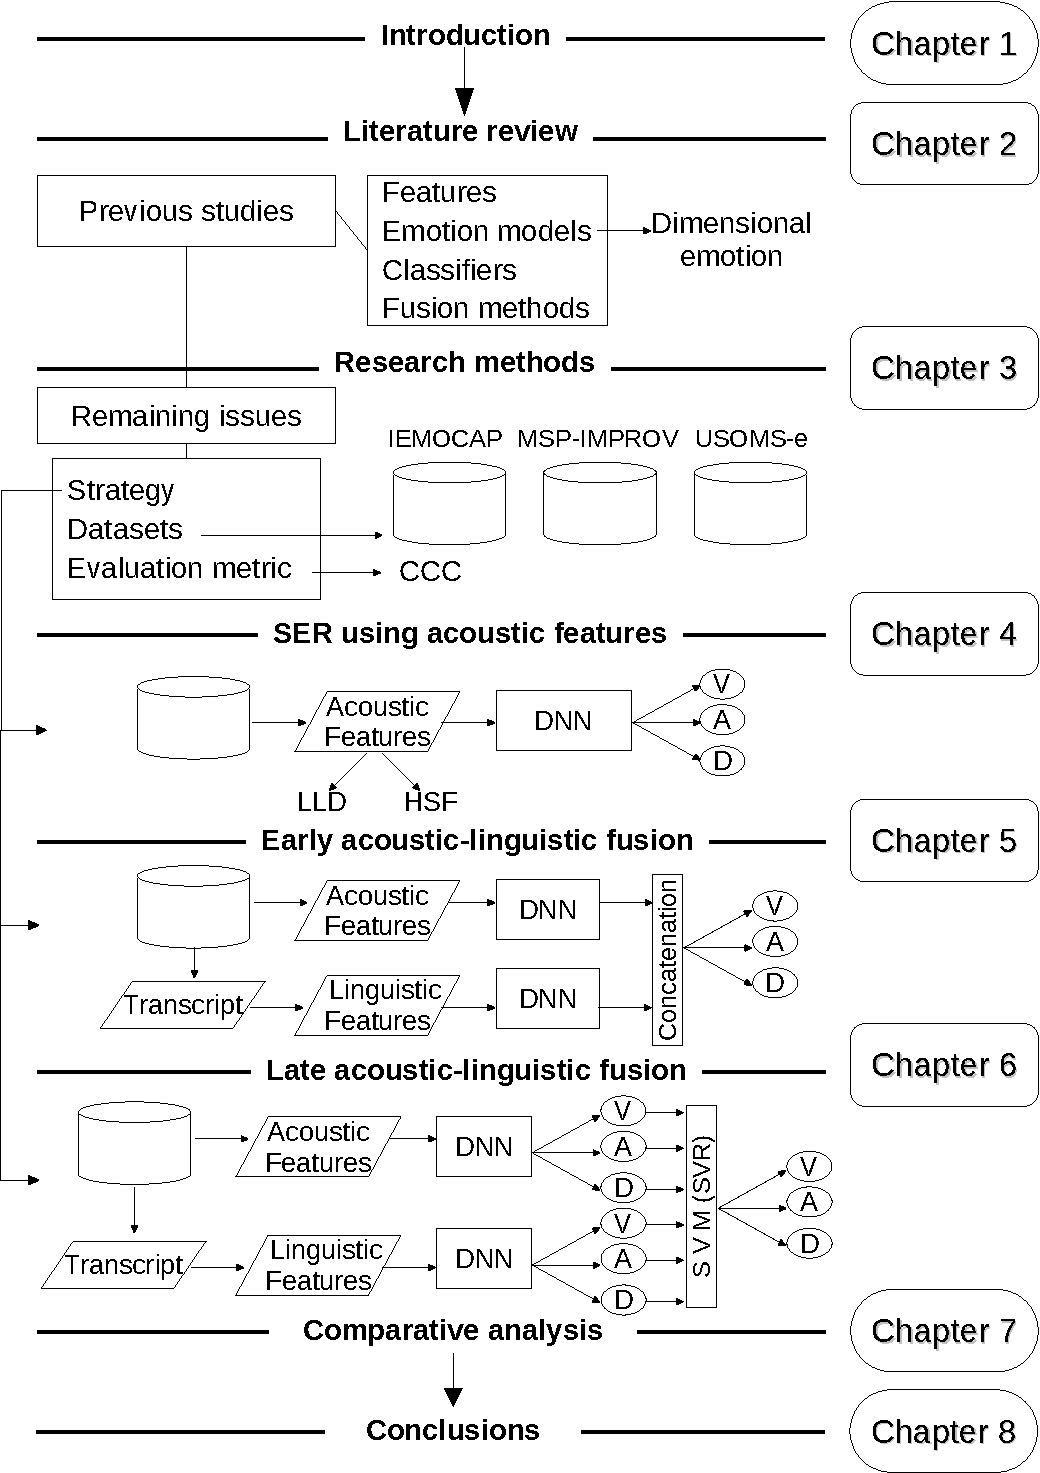
\includegraphics[width=.95\textwidth]{../fig/dissertation_org-crop.pdf}
    \caption{Organization of the dissertation}
    \label{fig:dissertation_org}
\end{figure}

% \newpage
% \thispagestyle{empty}
% \mbox{}
